% !TEX root = A0.MiTFM.tex

\chapter{Arquitectura de defensa en profundidad propuesta}

La auditoría de Fase~0 ha evidenciado que el problema principal no se encuentra en el cifrado de Widevine, sino en los caminos que permiten alcanzar el contenido y el servicio de licencia sin conservar el contexto de autorización. A partir de este resultado se propone una arquitectura incremental: Fase~1 introduce controles preventivos alrededor del DRM y Fase~2 añade persistencia, detección y respuesta. La finalidad no es reemplazar Widevine, sino impedir que una licencia técnicamente válida se obtenga fuera de una reproducción autorizada y aportar capacidad de reacción cuando el uso deja de ser coherente con la política del servicio.

Este capítulo presenta las decisiones de diseño de ambas fases. La implementación concreta se describe en el capítulo siguiente y la comparación experimental con Fase~0 se ha realizado en el Capítulo~7. Esta separación evita convertir la descripción arquitectónica en una enumeración de pruebas y permite justificar cada control por la debilidad que pretende corregir.

\section{Objetivos de la arquitectura defensiva}

La propuesta parte de cinco requisitos derivados directamente de los hallazgos F0-01 a F0-05. En primer lugar, todo camino capaz de entregar el manifiesto, el contenido local o una licencia debe exigir autorización; eliminar la ruta \texttt{/license/no\_auth} no sería suficiente si permaneciera otro acceso equivalente. En segundo lugar, el origen y el servidor de licencias no deben estar publicados directamente en el anfitrión. En tercer lugar, la identidad autenticada debe transformarse en una sesión de reproducción específica y efímera. En cuarto lugar, las peticiones deben vincularse a cuenta, dispositivo, instancia de cliente, activo y sesión, de modo que una credencial válida para un contexto no pueda trasladarse sin más a otro. Finalmente, el sistema debe conservar señales suficientes para detectar patrones anómalos y revocar el acceso.

Estos requisitos se traducen en tres propiedades verificables. La primera es \emph{consistencia}: manifiesto, contenido, heartbeat y licencia deben referirse a la misma sesión. La segunda es \emph{temporalidad}: el permiso de reproducción debe caducar si el cliente deja de mantener la sesión. La tercera es \emph{capacidad de respuesta}: una cuenta o dispositivo bloqueado no debe poder continuar utilizando una credencial emitida con anterioridad.

La arquitectura se mantiene deliberadamente acotada. No pretende construir un proveedor de identidad, un CDN comercial o una plataforma antifraude basada en aprendizaje automático. Su objetivo es materializar controles observables y reproducibles con los que comparar las tres fases del laboratorio.

\section{Modelo \textit{Defense in Depth} aplicado a OTT}

La defensa en profundidad se aplica como una composición de capas con responsabilidades distintas. El cliente inicia el flujo, pero no decide por sí mismo si el acceso es válido. Varnish reduce la superficie HTTP y normaliza la información de entrada. El \textit{control-plane} aplica identidad, \textit{entitlement}, sesión y contexto. El estado de Fase~2 permite relacionar peticiones separadas en el tiempo. Finalmente, el origen y el servidor de licencias permanecen internos y reciben únicamente solicitudes ya autorizadas.

La Figura~\ref{fig:arquitectura-defensa-capas} resume esta distribución. Fase~1 concentra la prevención: elimina el bypass, protege manifiesto, contenido local y licencia, y limita la concurrencia. Fase~2 incorpora memoria y respuesta: registra eventos, mantiene contadores, calcula riesgo y aplica bloqueos. Widevine continúa ocupándose del procesamiento de la licencia y de la protección de las claves dentro del CDM; las capas anteriores determinan si el flujo que llega hasta él es legítimo.

\begin{figure}[htbp]
    \centering
    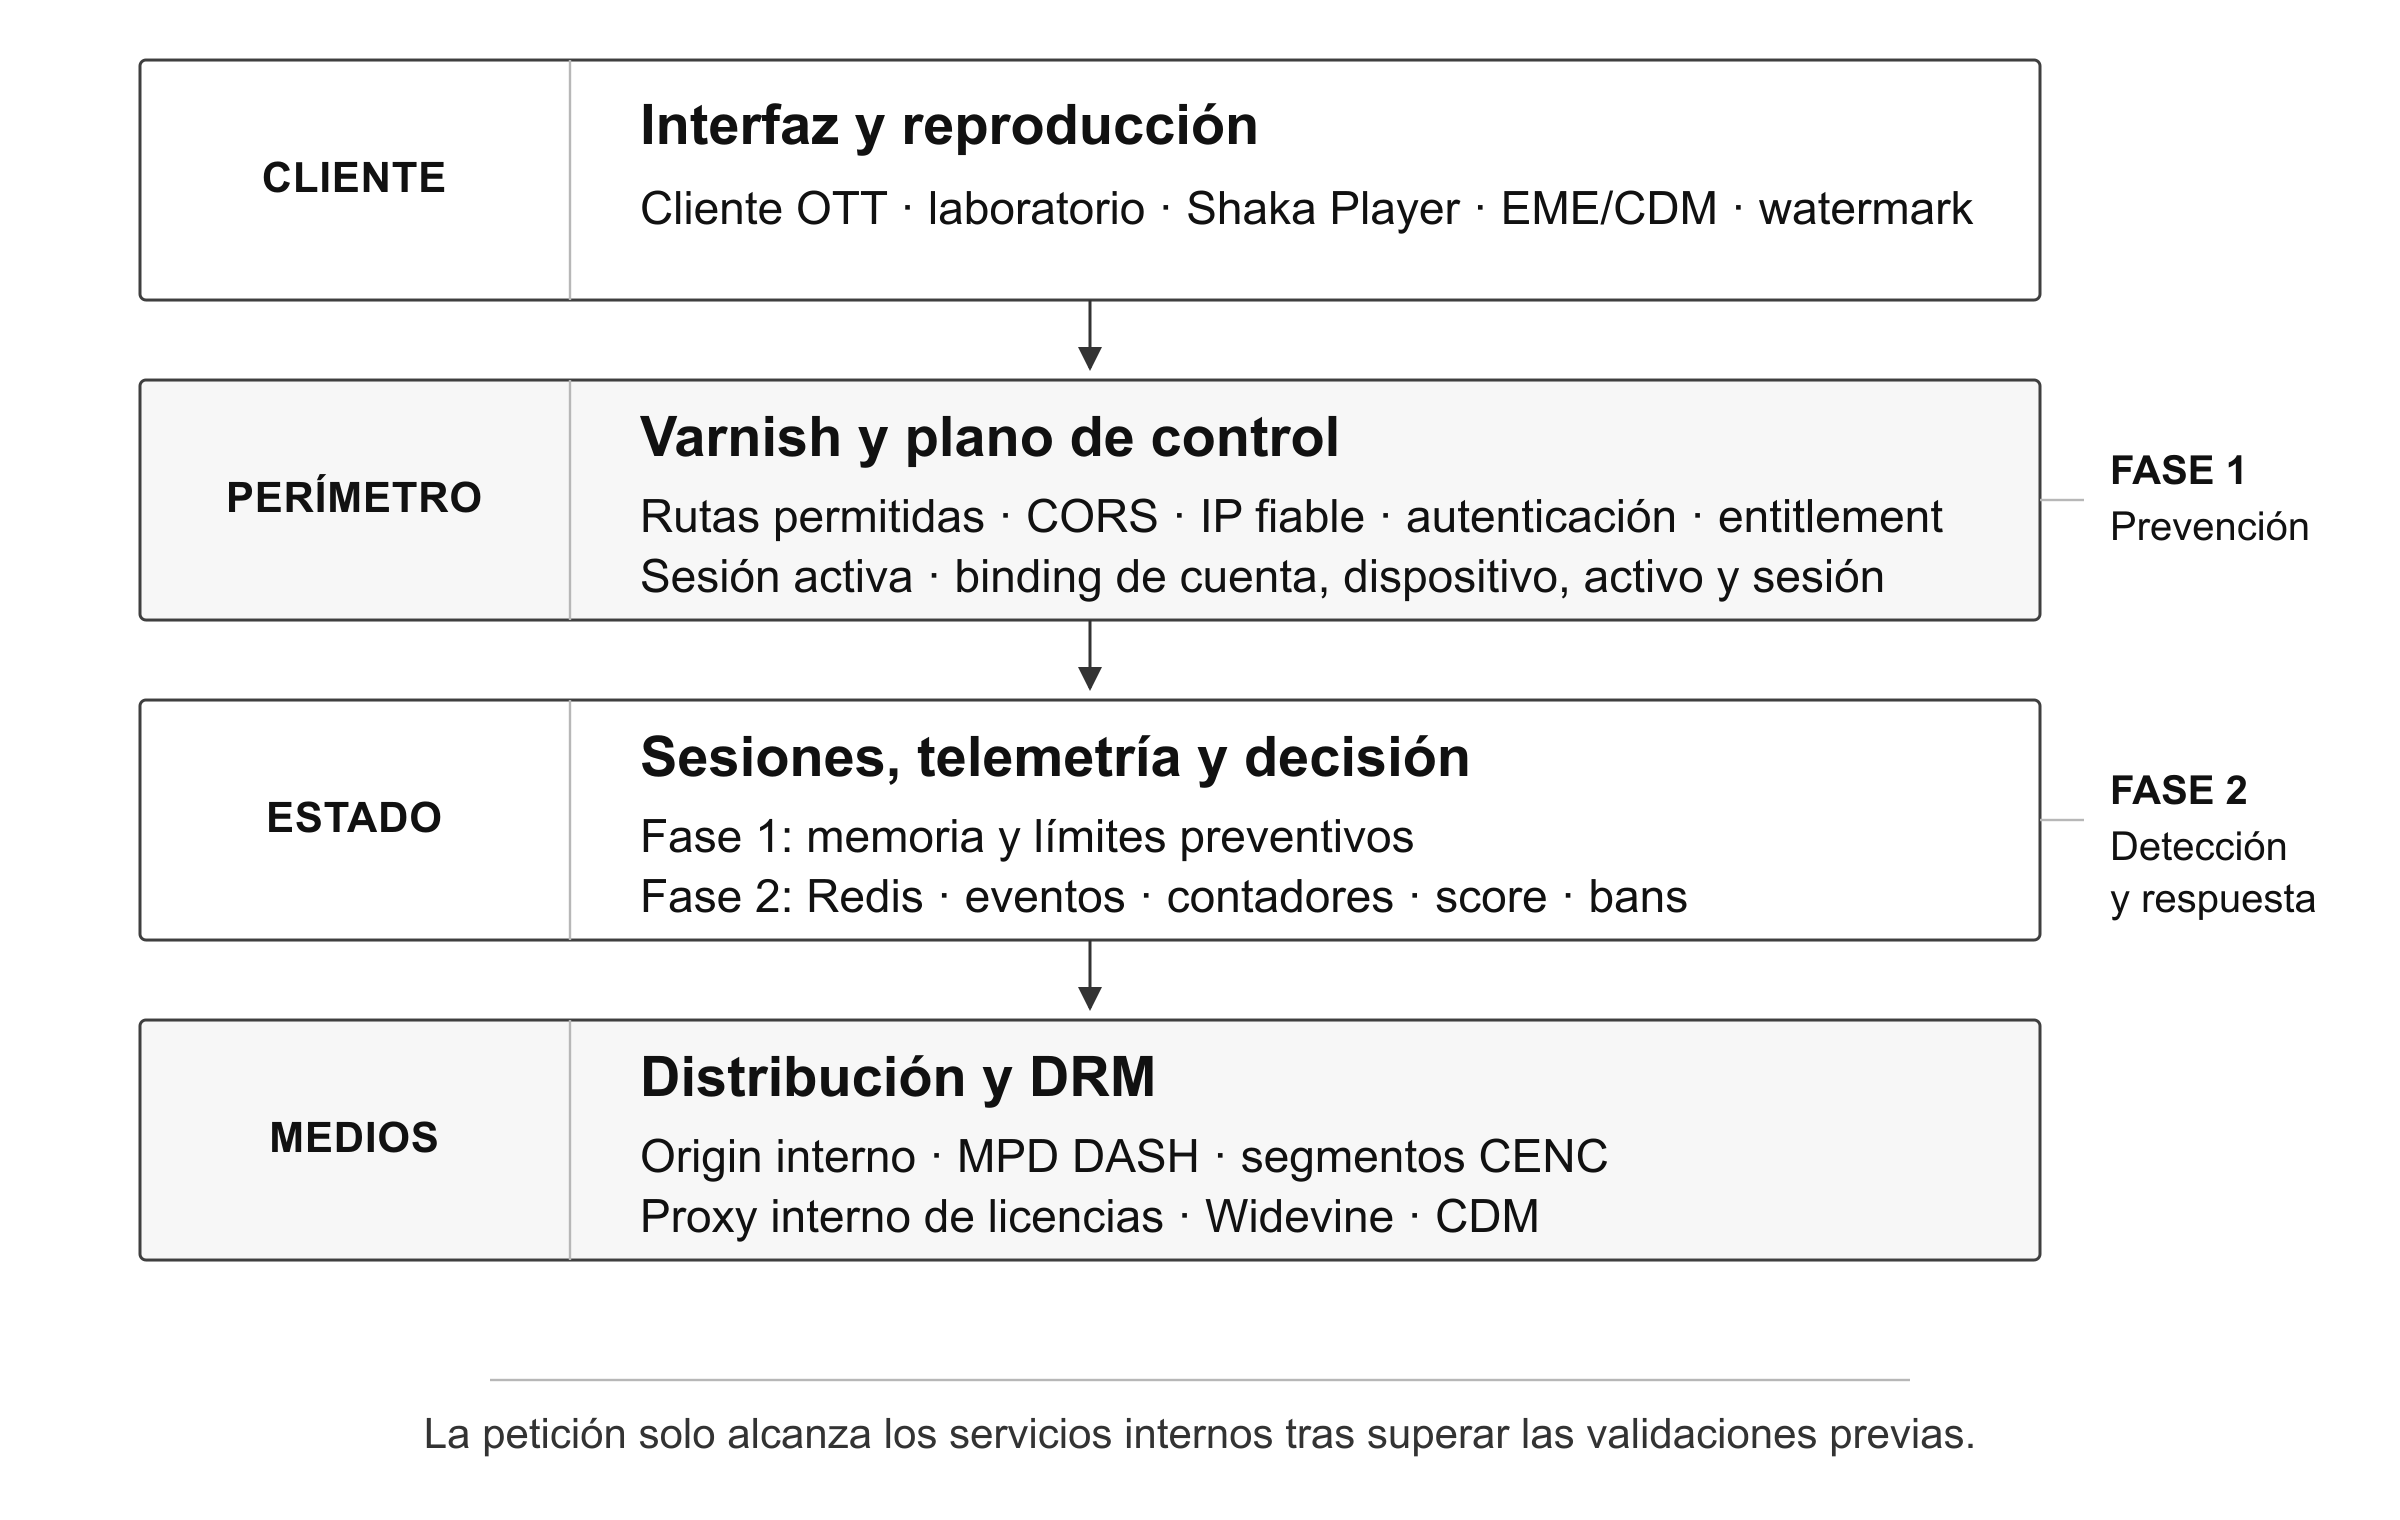
\includegraphics[width=0.98\textwidth]{figuras/arquitectura-defensa-capas.png}
    \caption{Capas de la arquitectura defensiva y responsabilidades de Fase~1 y Fase~2.}
    \label{fig:arquitectura-defensa-capas}
\end{figure}

La Tabla~\ref{tab:trazabilidad-controles} relaciona los problemas principales de Fase~0 con los controles propuestos. Esta trazabilidad es importante porque evita atribuir a una única medida una protección que depende de varias capas.

\begin{table}[H]
\centering
\caption{Trazabilidad entre hallazgos y controles defensivos}
\label{tab:trazabilidad-controles}
\begin{tabularx}{\textwidth}{p{0.15\textwidth}Yp{0.23\textwidth}}
\toprule
\textbf{Hallazgo} & \textbf{Control principal} & \textbf{Fase} \\
\midrule
Licencia pública & Único endpoint público de licencia, protegido por una sesión de reproducción. & Fase~1 \\
Origen y contenido expuestos & Servicios internos y autorización sobre manifiesto, segmentos y licencia. & Fase~1 \\
Sesión sin caducidad ni contexto & Credencial efímera ligada a cuenta, dispositivo, activo e instancia. & Fase~1 \\
Sin control de concurrencia & Límite preventivo y registro de rechazos reiterados. & Fases~1 y 2 \\
CORS y HTTP permisivos & Orígenes web restringidos; TLS reservado al despliegue de producción. & Fase~1 / producción \\
\bottomrule
\end{tabularx}
\end{table}

\section{Diseño del acceso protegido a manifiestos y licencias}

La Fase~0 permitía obtener el MPD y alcanzar el proxy Widevine mediante caminos que no compartían una política común. La propuesta unifica ambos recursos sensibles detrás del \textit{control-plane}. El cliente ya no recibe directamente el manifiesto público como configuración de reproducción, sino una URL local de la forma \texttt{/manifest/:assetId}. De igual modo, el único endpoint de licencia expuesto es \texttt{/license}; la ruta \texttt{no\_auth} desaparece del perímetro.

Esta decisión no convierte el MPD en una credencial secreta. Su función es asegurar que la plataforma compruebe el contexto antes de entregar la descripción de la presentación y de iniciar el flujo EME. En el activo Widevine público, los segmentos continúan alojados en la infraestructura de demostración de Shaka. Para los activos locales, la ruta \texttt{/content/*} aplica además una relación entre el activo del token y el prefijo permitido del origen.

\subsection{Interceptación}

Varnish constituye el único punto de entrada hacia el plano de control. Rechaza rutas no contempladas por la fase, exige la cabecera \texttt{Authorization} en manifiesto, contenido, licencia, heartbeat y parada de sesión, y genera un identificador de petición. Además, sustituye cualquier \texttt{X-Forwarded-For} aportado por el cliente por la dirección observada en la conexión. Con ello se evita que una señal de red utilizada para correlación pueda ser elegida libremente desde el navegador.

La interceptación también se produce en Shaka Player. El cliente añade el token de reproducción y las cabeceras de sesión, dispositivo e instancia a las solicitudes protegidas de manifiesto, contenido local y licencia. Se mantiene así una política común sobre recursos que Fase~0 trataba de manera independiente.

\subsection{Validación}

El \textit{control-plane} valida primero la firma y expiración de la credencial. Después comprueba que su tipo sea de reproducción y recupera la sesión indicada. La sesión debe existir, permanecer activa y coincidir con la cuenta, dispositivo, instancia de cliente y activo incluidos en el token. Finalmente, los identificadores declarados en las cabeceras deben concordar con el token y el activo solicitado debe coincidir con la ruta.

La Figura~\ref{fig:flujo-reproduccion-protegida} representa el flujo completo. La autenticación genera una credencial de acceso; esta permite crear una sesión y obtener una credencial de reproducción de corta duración. Solo la segunda se utiliza para solicitar el MPD y la licencia. El heartbeat renueva el permiso mientras la sesión permanece activa.

\begin{figure}[htbp]
    \centering
    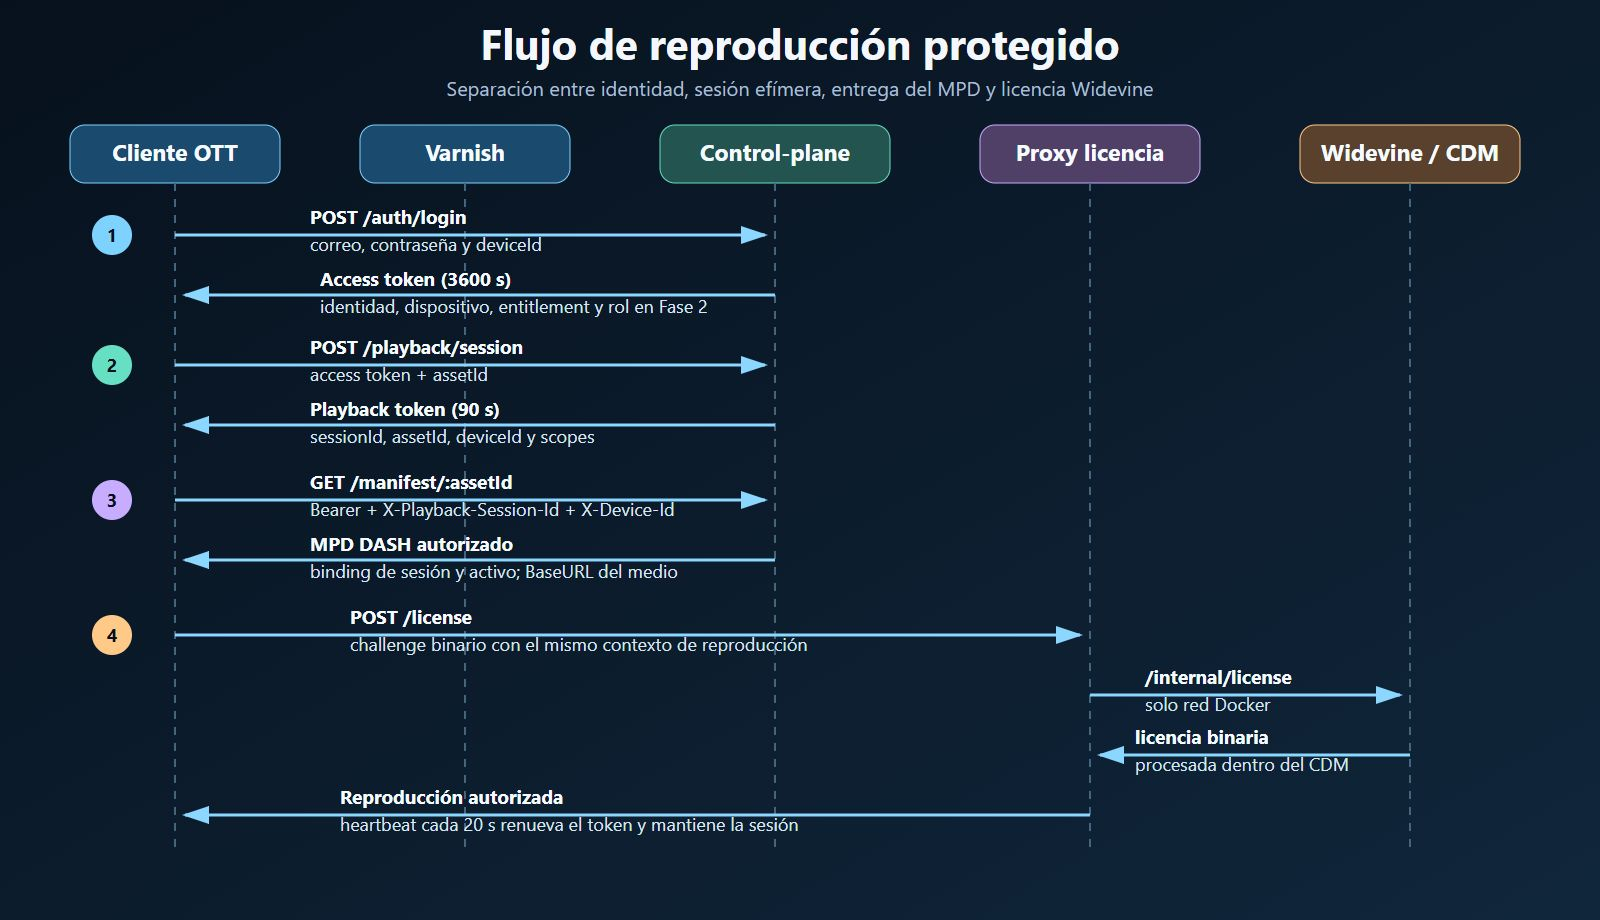
\includegraphics[width=0.98\textwidth]{figuras/flujo-reproduccion-protegida.png}
    \caption{Secuencia de autenticación, sesión, manifiesto y licencia en las fases endurecidas.}
    \label{fig:flujo-reproduccion-protegida}
\end{figure}

La validación se repite en cada punto sensible; no se asume que una decisión adoptada al crear la sesión siga siendo válida indefinidamente. Esta propiedad permite que una sesión detenida, expirada o bloqueada deje de servir aunque el cliente conserve una copia del token.

\subsection{Política de acceso}

La política distingue autenticación, autorización y reproducción. Un usuario puede presentar credenciales correctas y, aun así, carecer del \textit{entitlement} del activo. En ese caso obtiene identidad, pero la creación de la sesión se rechaza. Del mismo modo, disponer de un token de acceso no permite solicitar directamente manifiesto o licencia porque ambos endpoints exigen una credencial de tipo reproducción.

Las decisiones principales producen respuestas diferenciadas: ausencia o alteración de token implica rechazo de autenticación; un activo distinto al autorizado produce un error de autorización; una cabecera de sesión incoherente se trata como conflicto de contexto; y una segunda reproducción simultánea supera el límite de concurrencia. La codificación exacta de estas respuestas se describe en el capítulo de implementación y su comportamiento se ha evaluado en el Capítulo~7.

\subsection{CDN leeching y clave conocida}

La protección del servidor de licencias no basta cuando una clave ya ha salido del entorno previsto. En ese escenario, un tercero puede intentar obtener el MPD y los segmentos cifrados para reproducirlos en otro cliente o utilizarlos como fuente de un servicio de \textit{restreaming}. Por este motivo, el activo CENC local se publica en las fases endurecidas mediante el mismo plano autorizado: tanto el manifiesto como cada objeto de contenido exigen token, sesión, activo e instancia coherentes.

CORS se conserva como una limitación adicional para navegadores con un origen no permitido, pero no se considera un mecanismo de autenticación. Un cliente nativo o un backend IPTV no está obligado a aplicar la política del navegador y, si dispone de una sesión válida, puede realizar las solicitudes directamente. El control efectivo reside, por tanto, en la validación de servidor y no en la cabecera \texttt{Origin}.

Existe además un caso límite deliberadamente aceptado. Una única sesión legítima que presente un token vigente y la clave conocida puede descargar y reproducir un canal sin solicitar una nueva licencia. Bloquearla de forma inmediata produciría falsos positivos ante licencias ya disponibles en el dispositivo. Fase~2 trata la combinación de manifiesto y tres objetos de contenido sin petición de licencia como una señal heurística: añade 20 puntos una sola vez por sesión, pero no genera por sí sola un ban. La concurrencia, el cruce de activo, la copia desde otra instancia y el uso posterior a la parada continúan siendo rechazados de forma independiente.

\section{Sistema de autenticación y autorización}

\subsection{Credenciales de acceso y reproducción}

La arquitectura utiliza dos clases de credencial. El token de acceso representa la autenticación de la cuenta e incluye dispositivo, plan, permisos y, en Fase~2, roles. El token de reproducción representa una única sesión e incorpora cuenta, dispositivo, activo, \texttt{sessionId}, \texttt{clientInstanceId} y ámbitos para manifiesto, contenido, licencia y heartbeat.

Ambas credenciales se firman y disponen de expiración. El formato se ha simplificado para el laboratorio porque el aspecto evaluado no es un estándar concreto de identidad, sino la separación de privilegios, la vinculación con el contexto de reproducción y la posibilidad de revocar el acceso.

\subsection{Expiración y renovación}

La credencial de acceso tiene una vida mayor que la de reproducción. El diseño permite mantener una sesión de usuario razonable sin conceder durante el mismo periodo el acceso al plano de medios. El token de reproducción caduca rápidamente y se renueva mediante heartbeat. Si la aplicación deja de enviar esa señal, la sesión pasa a estado expirado y la siguiente validación falla.

La renovación no amplía una sesión que haya sido detenida o bloqueada. Antes de emitir el nuevo token se vuelve a recuperar el estado y, en Fase~2, se consulta también si existen bans de cuenta o dispositivo. Por tanto, la expiración corta limita la ventana de reutilización y el estado del servidor conserva la capacidad de revocar antes de que se alcance dicha expiración.

\subsection{Validación contextual}

El contexto mínimo se compone de cuenta, dispositivo, instancia de cliente, activo y sesión. La IP se utiliza como señal de correlación, no como identidad principal: puede cambiar por movilidad, NAT o infraestructura intermedia y no sería prudente bloquear automáticamente una cuenta por una única variación. La arquitectura tampoco afirma realizar geolocalización. Fase~2 conserva las IP observadas durante una ventana temporal y eleva el riesgo cuando una misma cuenta acumula actividad desde varias direcciones.

El identificador de dispositivo y el de instancia se generan en el cliente de laboratorio y se incluyen en las credenciales. Ninguno constituye una atestación criptográfica de hardware; su utilidad es hacer reproducible el binding, diferenciar una ejecución concreta y permitir demostrar el bloqueo de un sujeto. Un sistema comercial requeriría señales más resistentes a manipulación, pero esa ampliación no es necesaria para comprobar el efecto de la política propuesta.

\section{Controles de concurrencia y ciclo de vida}

\subsection{Límite de sesiones}

Antes de crear una sesión, el \textit{control-plane} cuenta las sesiones activas de la cuenta. El laboratorio fija el máximo en una reproducción simultánea. Si ya existe una, la segunda solicitud se rechaza sin emitir otro token de reproducción. El control se sitúa en la aplicación y no en Widevine, porque el DRM no conoce el número de reproducciones permitido por el plan contratado.

Fase~1 mantiene este estado en memoria. Fase~2 lo conserva en Redis, lo que permite que las comprobaciones de distintas peticiones consulten una fuente común y que la interfaz administrativa muestre sesiones recientes. En ambos casos, el estado incluye inicio, último heartbeat, cuenta, dispositivo, instancia de cliente, activo y situación de la sesión.

\subsection{Correlación de IP y dispositivo}

La dirección observada por Varnish se asocia a los eventos de autenticación y creación de sesión. Fase~2 mantiene durante diez minutos el conjunto de IP recientes por cuenta y lo utiliza como una señal de riesgo. El dispositivo y la instancia permanecen en el token y en la sesión, por lo que trasladar únicamente la credencial y modificar una cabecera no produce un contexto coherente.

Esta correlación no equivale a afirmar que cada IP identifica una persona ni que el \texttt{deviceId} sea imposible de copiar. La defensa surge de combinar señales y de repetir la validación, no de confiar de manera absoluta en un único atributo controlado parcialmente por el cliente.

\subsection{Expiración y finalización}

La sesión puede terminar de tres maneras. La aplicación puede detenerla explícitamente mediante \texttt{/playback/stop}; puede expirar al superar la gracia sin heartbeat; o puede quedar inutilizable al aparecer un ban aplicable. La separación entre estado de sesión y token permite que conservar una credencial no sea suficiente para restaurar ninguna de estas situaciones.

\section{Detección de anomalías}

\subsection{Patrones sospechosos}

Fase~2 observa señales que pueden relacionarse con abuso: actividad de una cuenta desde varias IP, rechazos repetidos de concurrencia, ráfagas de licencias, tasas elevadas de contenido, contenido consumido sin una licencia observada en la sesión, heartbeats con una cadencia superior a la del cliente y fallos de autenticación concentrados en un dispositivo. Ninguna de estas señales demuestra por sí sola fraude; su función es producir una decisión reproducible dentro del experimento.

Los eventos conservan el tipo de operación, identificadores relevantes y marca temporal. Para las solicitudes de manifiesto y licencia se registra además la sesión y el riesgo calculado. Las claves Widevine y los tokens completos quedan fuera del registro, reduciendo el riesgo de que la propia observabilidad se convierta en una fuente de credenciales.

\subsection{Límites y contadores temporales}

Fase~1 incorpora límites preventivos por IP y ventana para autenticación, creación de sesión, manifiesto, heartbeat, contenido y licencia. Fase~2 utiliza contadores persistidos con TTL como señales de comportamiento. Esta segunda estrategia no se limita a devolver un error por volumen: acumula contexto y puede terminar en un ban.

Los umbrales se han elegido para facilitar escenarios de laboratorio y no proceden de una calibración con tráfico real. Por ello, la arquitectura separa su significado de la cifra concreta. El diseño relevante es la existencia de ventanas, contadores y una acción posterior; la adecuación estadística de cada umbral pertenece a una evaluación con una población de usuarios que queda fuera del alcance del prototipo.

\subsection{Correlación básica}

La correlación se realiza por cuenta, dispositivo, sesión e IP observada. Cada señal puede aumentar una puntuación y añadir una razón legible. Cuando la puntuación de cuenta alcanza el umbral configurado se crea un ban automático. Los fallos de autenticación siguen un camino más directo: al alcanzar la ráfaga definida se bloquea temporalmente el dispositivo, incluso aunque no exista una sesión autenticada desde la que calcular riesgo de cuenta.

La Figura~\ref{fig:flujo-deteccion-respuesta} resume el recorrido desde la señal hasta la respuesta. Redis mantiene el estado intermedio y el plano administrativo permanece separado del plano de reproducción, de modo que un operador pueda inspeccionar o retirar un bloqueo sin depender de que el dispositivo bloqueado siga autorizado.

\begin{figure}[htbp]
    \centering
    
\includegraphics[width=0.98\textwidth]{figuras/flujo-deteccion-respuesta.png}
    \caption{Flujo de eventos, riesgo y respuesta activa en Fase~2.}
    \label{fig:flujo-deteccion-respuesta}
\end{figure}

\section{Bloqueo y mitigación}

\subsection{Bans de cuenta y dispositivo}

La propuesta evita el baneo automático por IP como mecanismo principal. Una dirección puede representar varios usuarios o cambiar sin que exista abuso. Los sujetos bloqueables son la cuenta y el dispositivo: la primera agrupa el comportamiento autenticado y el segundo permite responder a una ráfaga de fallos previa al login. Las IP permanecen como contexto de detección.

Los bans son temporales y contienen motivo, creador, instante de creación y expiración. Pueden generarse automáticamente o desde el plano administrativo. La validación de bans se ejecuta tanto con tokens de acceso como con tokens de reproducción, por lo que afecta al login posterior y a las operaciones de una sesión ya creada.

\subsection{Revocación y recuperación}

El sistema diferencia el plano de reproducción del plano administrativo. Los endpoints de observabilidad y gestión requieren un token de acceso con rol \texttt{admin}, pero no dependen de que el dispositivo mantenga permiso para reproducir. Así se evita que aplicar un ban deje al operador sin capacidad para observarlo o retirarlo.

La revocación no borra la evidencia: la creación y la retirada producen eventos separados. Una vez eliminado el ban, el cliente debe volver a superar la validación y renovar el token de reproducción antes de continuar. Esta recuperación explícita permite demostrar que el bloqueo no consiste únicamente en deshabilitar un botón de la interfaz.

\subsection{Invalidación de sesión}

Detener una sesión cambia su estado y provoca que cualquier token asociado sea rechazado. La expiración por ausencia de heartbeat produce el mismo efecto. Ante un ban, la sesión puede permanecer registrada para trazabilidad, pero deja de ser utilizable porque la comprobación del sujeto bloqueado precede a la entrega de manifiesto, contenido o licencia.

\section{Arquitectura final integrada}

La arquitectura final combina prevención, detección y respuesta sin trasladar al DRM responsabilidades que pertenecen a la plataforma. Fase~1 elimina caminos alternativos, internaliza origen y licencia, separa identidad de reproducción y exige un contexto coherente. Fase~2 añade persistencia efímera, eventos estructurados, reglas de riesgo, bans y una interfaz administrativa.

El resultado conserva una propiedad esencial para el TFM: las tres fases siguen siendo comparables. Fase~0 permite observar el flujo vulnerable; Fase~1 muestra el efecto de aplicar autorización extremo a extremo; y Fase~2 permite estudiar qué aporta la memoria del comportamiento una vez corregido el bypass básico. El capítulo siguiente describe cómo se ha materializado esta arquitectura en Docker, Node.js, Varnish, Redis, Shaka Player y los laboratorios de auditoría.
